%%%%% METHODS %%%%%

\begin{figure*}[htbp]
    \centering
    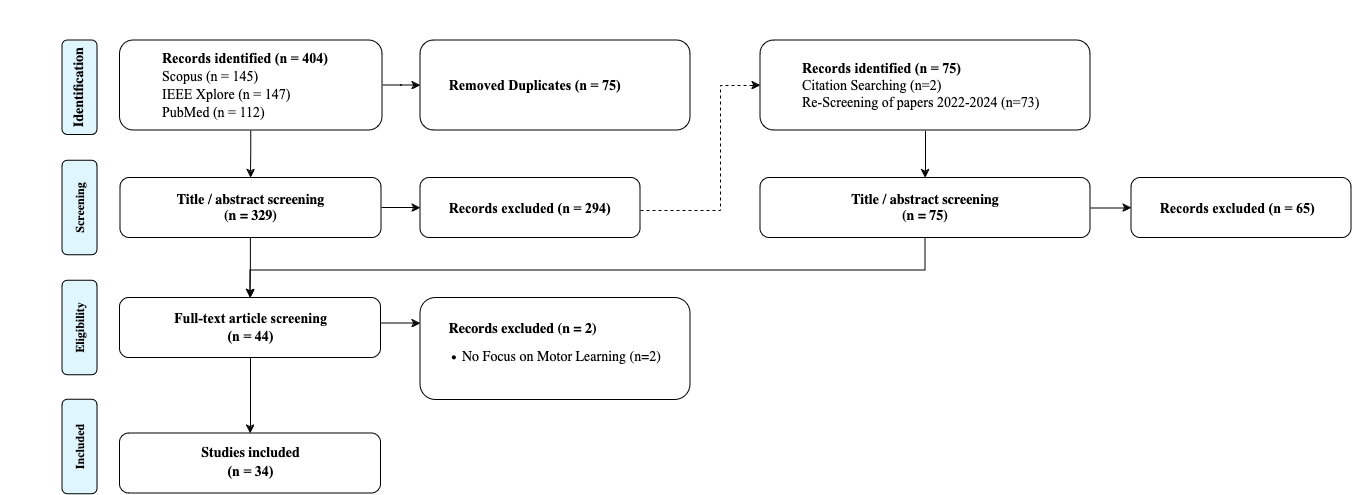
\includegraphics[width=\linewidth]{figures/prisma_overview.png} 
    \caption{Overview of the methodology using the PRISMA method}
    \label{fig:prisma}
\end{figure*} 

\section{Methods}

The method of the systematic review was based on the PRISMA methodology \cite{Page2021TheReviews} to ensure transparent and complete reporting on the topics examined.

\subsection{Search Strategy and Eligibility Criteria}
\label{sec:eligibility}
Several relevant articles were reviewed at the beginning to find eligible search terms. The query based on the research question consists of three main parts, namely \textit{virtual reality}, \textit{somatosensory feedback}, and \textit{motor learning}, each term with their respective synonyms. 

The final search query was as follows: motor AND (learning OR control OR training OR skills) AND (((virtual OR augmented) AND reality) OR ((remote OR virtual OR simulated) AND environment)) AND (((somatosensory OR haptic OR tactile OR proprioceptive OR kinesthetic OR cutaneous OR somatic) AND 
(cue* OR feedback OR rendering OR stimul*)) AND (fidelity OR realism OR accuracy OR precision OR exactness OR specificity)). The search terms were applied for the article title, abstract, and keywords.

Three databases (Scopus, IEEE Xplore, and PubMed) were searched in April 2024. Based on the required syntax of each database, the search query was slightly adapted. For example, as PubMed only allows for the use of an asterisk for words containing more than three letters, the term \textit{cue*} was changed to (\textit{cue} OR \textit{cues}). The exact search queries can be found in \ref{sec:queries}. 

To qualify for inclusion, studies had to focus on the impact of somatosensory feedback on motor learning in humans. We included studies with healthy participants only, as patients often know how to perform a movement but are physically constrained by their condition, therefore augmented feedback may help the motor learning of patients in a different way compared to healthy subjects \cite{Sigrist2013AugmentedReview}. There were no publication date or language limits.

Conversely, studies were excluded if they (i) did not relate to motor learning in humans; (ii) focused on systems not providing haptic feedback in VR; (iii) were concerned with a neurological condition affecting motor learning; or (iv) explained a new assessment system for the evaluation of motor learning.

\subsection{Study Selection}
At first, duplicate publications were identified and removed. The results were then screened based on their title and abstract. 

In this review, we wanted to emphasize more recent studies to reflect the significant impact of recent technological advances in VR on the field. Therefore, records published in the years 2022-2024 were re-screened and also included in the further process, if they were only partially fitting the eligibility criteria. Additional papers were identified using citation searching.

Finally, the full-text articles were assessed to determine their eligibility for inclusion in the review (see fig. \ref{fig:prisma}).


\section{Search Results}

%%%% Rewrite for precise numbers!! %%%%%

The search yielded a total of 404 results, which were saved in the library of Mendeley. 75 duplicates were found and removed. The remaining 329 records were screened based on title and abstract first. This led to the preliminary exclusion of 294 records, of which 73 records were re-screened as they were from the years 2022-2024 (see fig. \ref{fig:prisma}). 
Additionally, 2 papers were included based on citation search. 

In total, 44 articles were full-text screened. Out of these, 7 were excluded based on the exclusion criteria described in \ref{sec:eligibility}, and the remaining 34 studies were included in this review.


\subsection{Study characteristics}

\subsubsection{Year of publication}
The year of publication of the included studies ranges from 2000 to 2024. As seen in \ref{fig:years}, the number of studies has greatly increased in the past decade, with a peak in 2018.

\begin{figure}[htbp]
    \centering
    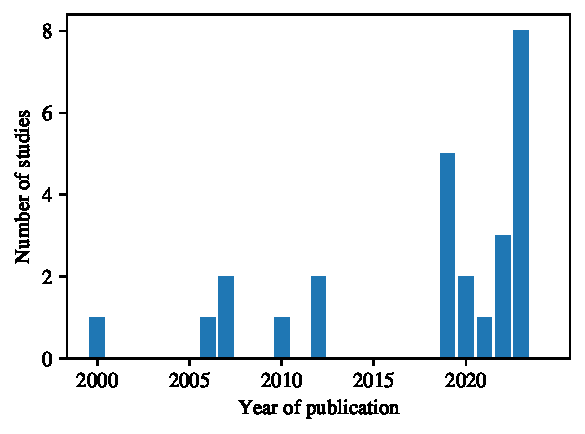
\includegraphics[width=\columnwidth]{figures/years.pdf} 
    \caption{Publication dates of the included articles}
    \label{fig:years}
\end{figure} 

\subsubsection{}


\section{Definitions}
\subsection{Fidelity}
Huang et al. suggested that skill transfer might be a useful paradigm to evaluate the level of fidelity, assuming that if an environment has infinite fidelity and is therefore perfectly recreating the sensations of the real environment, then there would be no performance loss when transferring the skill from the virtual to the real environment \cite{Huang2006}

\section{Somatosensory feedback}
\subsection{Low-fidelity feedback}

\subsection{Mid-fidelity feedback}
Even though it is not labeled as such, Morris et al. conducted an experimental study in which they provided mid-fidelity feedback to the participants. They were asked to follow a trajectory with a haptic device stylus, and in the first condition of the experiment the device provided force feedback that was pointing in the opposite direction as the trajectory, while the participants were asked to keep the device in the movement plane, so to counteract the applied force exactly \cite{Morris2007}. While participants applied the same force necessary to follow the trajectory, the movement and position control differed from actually following the pattern.



\subsection{High-fidelity feedback}
Huang et al. showed in an experiment that high-fidelity feedback can be helpful in controlling an external dynamic system, as it enhances performance during online control \cite{Huang2007}. The subjects were asked to excite a spring-inertia system with maximum amplitude, which could be achieved by leveraging the resonance frequency of the system and therefore increasing its oscillations. When haptic feedback was provided, the participants were more precise in finding the frequency and decreased their variability.

Haptic guidance specifically can help in the temporal aspects of learning a task \cite{Feygin2002HapticSkill} 

\subsection{Framework}

\subsubsection{Hardware precision}
"The required refresh rate to provide realistic
force feedback is commonly accepted to be at least 1,000 Hz.
However, this refresh rate is widely debated. According to
Burdea [14], a minimum refresh rate of only 300 Hz is
acceptable. Conversely, a study by Booth et al. [15] using
SensAble’s Premium 1.5 to deduce the minimum acceptable
haptic refresh rate, suggests that “a minimum acceptable
refresh rate must lie within the 550-600 Hz range.” The
necessary rate of update is dependent upon the stiffness of
the surfaces to be simulated. A stiff contact between objects is
better simulated by higher refresh rates, whereas lower
refresh rates are satisfactory for softer objects. Additional
methods can be applied to simulate touching stiffer objects
such as combining vibrations with force to the end effector to
represent the small vibrations felt upon object contact [16].
Typically, a trade-off must be made between the accuracy of
the haptics effects produced and the speed required within
the application." \cite{Coles2011TheArt}
About latency and its impacts: \cite{Gourishetti2018PassiveFeedback}.
Ballistic movements: rapid, involuntary movement which is motor programmed, and for which visual feedback is not possible \cite{Wall2000}.
